


\chapter{Optimized \acs{DSPG} Synthesis and Trust Network Analysis with Subjective Logic [By End of March]}
\label{chap:tnasl}
\todo[inline]{Should I mention that this chapters are based on my papers where I contributed with others}
\todo[inline]{Add Evaluation to show the time complexity, especially the Nesting Level Computation}
\section{Introduction}

\acf{TNA-SL}, introduced by J{\o}sang~\cite{10.5555/1151699.1151710}, enables trust reasoning under uncertainty by propagating and aggregating subjective opinions along graph structures. In the methodology introduced in \cref{chap:Trust_method}, \ac{TNA-SL} is used on \ac{STN} to generate the expression in phase I. However, as discussed in \cref{sec:dspg}, a fundamental structural requirement of \ac{TNA-SL} is that the underlying trust network must be a \ac{DSPG}. This structural constraint ensures that trust propagation through discounting and fusion operators is well-defined and yields unambiguous results.

In practice, real-world trust networks rarely satisfy the \ac{DSPG} property. In practical applications trust relationships form complex directed acyclic graphs that contain structural patterns incompatible with DSPG constraints. Consequently, a transformation step, commonly referred to as \ac{DSPG} synthesis, is required prior to trust inference.

\ac{DSPG} synthesis approach proposed in the original work of J{\o}sang~\cite{10.5555/1151699.1151710} incrementally adds branches while verifying structural criteria. 
% As formalized in~\cite{10.1007/978-3-032-08887-1_4}, 
This method relies on overly restrictive conditions and often remove edges considered structurally unsafe. Although this guarantees DSPG compliance, it introduces two major limitations.
\begin{enumerate}
    \item \textbf{Information loss.} Structurally meaningful trust relationships may be discarded, even when they do not fundamentally violate the \ac{DSPG} requirements.
    \item \textbf{Misaligned optimization objective.} Prior approaches implicitly assume that minimizing uncertainty should be the primary objective of synthesis. In practice, preserving as much structural information as possible should be the primary objective.
\end{enumerate}

These observations reveal a structural inefficiency in existing DSPG synthesis methods. The criteria are overly conservative, and the transformation objective is not aligned with information preservation.

At the same time, the \ac{DSPG} analysis phase performed after synthesis suffers from a computational inefficiency. The classical \ac{TNA-SL} reduction (\ac{DSPG} analysis) procedure repeatedly recomputes the \acf{NL} of edges a after each structural transformation. Since \acp{NL} determine the order in which \acp{PPS} are reduced, each reduction step requires a global recomputation of \acp{NL} across the graph. For large trust networks this leads to significant computational overhead and limits the scalability of the analysis procedure.

Finally, classical \ac{SL} trust discounting operators, namely the Two-Edge Path and Multi-Edge Path operators (\cref{table:TD_operators}), assume that the final edge of a path represents functional direct trust. As illustrated in the \ac{IMA} use case, certain network topologies require the discounting of referral-only paths during the reduction process. However, the existing trust discounting operators assume that the final edge of a path represents functional direct trust, which prevents their consistent application in such cases.

Therefore, the limitations of \ac{TNA-SL} are threefold:
\begin{itemize}
    \item A structural limitation caused by overly restrictive \ac{DSPG} synthesis criteria.
    \item An operator-level limitation caused by incomplete trust discounting semantics for referral-only paths.
    \item A computational limitation arising from the repeated recomputation of edge \acp{NL} during \ac{DSPG} analysis, which increases the time complexity of trust inference.
\end{itemize}

This chapter addresses the three aspects in a unified framework.

\subsection*{Unified Optimization Perspective}

We propose an improved \ac{TNA-SL} framework that improves computational efficiency, preserves information, and ensures discounting consistency.

The contributions of this chapter are fourfold.

\begin{enumerate}
    \item \textbf{Refined structural characterization via \ac{PNPS}.} We introduce the concept of \acf{PNPS}, which refines the classical definition of \acf{PPS}. This reformulation provides stronger structural guarantees and enables more efficient detection of DSPG violations.

    \item \textbf{Optimized \ac{DSPG} synthesis criteria.} We derive revised synthesis criteria that admit a strictly larger class of edges while preserving \ac{DSPG} compliance. Unlike prior strategies, the proposed approach prioritizes maximal information retention during synthesis.
    
    \item \textbf{Optimized \ac{DSPG} analysis algorithm.}
    By operating on \ac{PNPS} structures rather than \ac{PPS}, the proposed algorithm ensures structural isolation during reductions and streamlines the computation of \acp{NL}, thereby reducing unnecessary recomputations. We formally establish the corresponding \ac{NL} preservation properties.
    \todo[inline]{add: Optimized algorithm  for DSPG Synthesis, }

    \item \textbf{Referral-edge path discounting operator.} To resolve inconsistencies in referral-only chains, we introduce a novel trust discount operator that extends \ac{SL} discounting semantics to paths composed entirely of referral edges. The proposed operator is compatible with existing Two-Edge and Multi-Edge operators and preserves expected trust attenuation properties across increasing path lengths~\cite{10706345}.
\end{enumerate}
Taken together, these contributions make \ac{TNA-SL} more general, more information-preserving, and more computationally efficient. As a result, the framework becomes better suited for complex systems such as \acp{NN}, where trust must be propagated across heterogeneous and potentially unreliable information sources.

The remainder of this chapter formalizes the proposed framework. Section~\ref{sec:pnps} introduces the \ac{PNPS} concept and the associated structural reformulation.  Section~\ref{sec:optimized_criteria} presents the optimized \ac{DSPG} synthesis criteria. Section~\ref{sec:optimized_analysis} details the optimized analysis algorithm and establishes its correctness properties. Section~\ref{sec:referral_path_operator} introduces the new referral-edge discount operator and analyzes its compatibility with classical Subjective Logic operators. Section~\ref{sec:eval_tnasl} presents the evaluation. Finally, Section~\ref{sec:summary_tnsl} concludes the chapter.

\section{Parallel Non-Intersecting Path Subnetworks}
\label{sec:pnps}

To address the limitations of \ac{DSPG} synthesis and analysis procedures identified in the introduction, we refine the notion of \ac{PPS} originally used in \ac{DSPG} analysis. While \ac{PPS} structures are sufficient for defining the classical \ac{DSPG} reductions order, they are not strong enough to guarantee structural isolation during analysis and \ac{NL} updates. 

For example, consider the graph shown in \cref{fig:ppsv}. If the \ac{PPS} between nodes \(A\) and \(C\) is reduced into a single edge \(AC\), the \ac{NL} of this newly created edge becomes \(0\), while the \acp{NL} of the remaining edges decrease by one. This global update illustrates that reductions based solely on \ac{PPS} structures do not preserve local structural isolation during the reduction process. To overcome this limitation, we introduce a stricter structural construct called the \acf{PNPS}. This refinement plays a central role in enabling both a clearer formalization of \ac{DSPG} structures and stable \ac{NL} computation after \ac{PNPS} reduction into a single edge.

\begin{definition}[\aclu{PNPS}]
\label{def:pnps}
Let $(A,B)$ be a \aclu{PPS} (\cref{def:pps}). It is called a \ac{PNPS} if and only if there exist at least two non-intersecting directed paths from the source $A$ to the sink $B$.
\end{definition}
The key difference between \ac{PPS} and \ac{PNPS} lies in the non-intersection requirement. This distinction is illustrated in \cref{fig:pnps}. For instance, although $(A,G)$ qualifies as a \ac{PPS}, it is not a \ac{PNPS} because we cannot find two non-intersecting paths between $A$ and $G$.

\begin{figure}[]
    \centering
    \begin{subfigure}{0.49\textwidth}
        \centering
        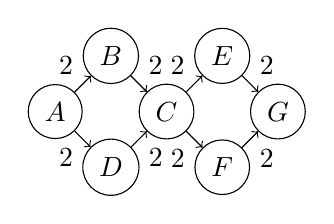
\begin{tikzpicture}[main/.style = {draw, circle}] 
        \node[main] (1) {$A$}; 
        \node[main] (2) [above right of=1] {$B$};
        \node[main] (3) [below right of=1] {$D$}; 
        \node[main] (4) [below right of=2] {$C$};
        \node[main] (5) [above right of=4]{$E$}; 
        \node[main] (6) [below right of=4] {$F$};
        \node[main] (7) [below right of=5] {$G$};
        \draw[->] (1) -- node[midway, above left]{2} (2);
        \draw[->] (1) --  node[midway, below left]{2} (3);
        \draw[->] (2) -- node[midway, above right]{2} (4);
        \draw[->] (3) -- node[midway, below right]{2} (4);
        \draw[->] (4) -- node[midway, above left]{2} (5);
        \draw[->] (4) --  node[midway, below left]{2} (6);
        \draw[->] (5) -- node[midway, above right]{2} (7);
        \draw[->] (6) -- node[midway, below right]{2}  (7);
        \end{tikzpicture}
        \caption{PPS edges NL before reduction}
        \label{fig:ppsv}
    \end{subfigure}
    \hfill
    \begin{subfigure}{0.49\textwidth}
        \centering
        \begin{tikzpicture}[main/.style = {draw, circle}] 
        \node[main] (1) {$A$}; 
        \node[main] (4) [below right of=2] {$C$};
        \node[main] (5) [above right of=4]{$E$}; 
        \node[main] (6) [below right of=4] {$F$};
        \node[main] (7) [below right of=5] {$G$};
        \draw[->, red] (1) -- node[midway, above]{0} (4);
        \draw[->] (4) -- node[midway, above left, text=red]{1} (5);
        \draw[->] (4) --  node[midway, below left, text=red]{1} (6);
        \draw[->] (5) -- node[midway, above right, text=red]{1} (7);
        \draw[->] (6) -- node[midway, below right, text=red]{1}  (7);
        \end{tikzpicture}
        \caption{PPS edges NL after reduction}
        \label{fig:ppsv}
    \end{subfigure}
    \hfill
    \begin{subfigure}{0.49\textwidth}
        \centering
        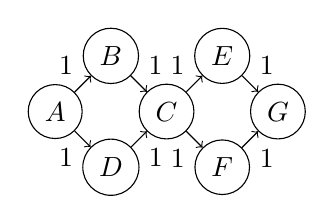
\begin{tikzpicture}[main/.style = {draw, circle}] 
        \node[main] (1) {$A$}; 
        \node[main] (2) [above right of=1] {$B$};
        \node[main] (3) [below right of=1] {$D$}; 
        \node[main] (4) [below right of=2] {$C$};
        \node[main] (5) [above right of=4]{$E$}; 
        \node[main] (6) [below right of=4] {$F$};
        \node[main] (7) [below right of=5] {$G$};
        \draw[->] (1) -- node[midway, above left]{1} (2);
        \draw[->] (1) --  node[midway, below left]{1} (3);
        \draw[->] (2) -- node[midway, above right]{1} (4);
        \draw[->] (3) -- node[midway, below right]{1} (4);
        \draw[->] (4) -- node[midway, above left]{1} (5);
        \draw[->] (4) --  node[midway, below left]{1} (6);
        \draw[->] (5) -- node[midway, above right]{1} (7);
        \draw[->] (6) -- node[midway, below right]{1}  (7);
        \end{tikzpicture}
        \caption{ \ac{PNPS} edges NL before reduction}
        \label{fig:pnpsv}
    \end{subfigure}
    \begin{subfigure}{0.49\textwidth}
        \centering
        \begin{tikzpicture}[main/.style = {draw, circle}] 
        \node[main] (1) {$A$}; 
        \node[main] (4) [below right of=2] {$C$};
        \node[main] (5) [above right of=4]{$E$}; 
        \node[main] (6) [below right of=4] {$F$};
        \node[main] (7) [below right of=5] {$G$};

        \draw[->, red] (1) -- node[midway, above]{0} (4);
        \draw[->] (4) -- node[midway, above left]{1} (5);
        \draw[->] (4) --  node[midway, below left]{1} (6);
        \draw[->] (5) -- node[midway, above right]{1} (7);
        \draw[->] (6) -- node[midway, below right]{1}  (7);
        \end{tikzpicture}
        \caption{ \ac{PNPS} edges NL after reduction}
        \label{fig:pnpsv}
    \end{subfigure}
    \caption{Comparison of \ac{PPS} and  \ac{PNPS}}
    \label{fig:pnps}
\end{figure}


% \subsection{Structural Characterization of Non-DSPG}

The introduction of  \ac{PNPS} enables a simplified structural characterization of non-\ac{DSPG} graphs.

\begin{proposition}[\ac{DSPG} Structural Constraint]
\label{prop:dspg}
A directed acyclic graph is not a \ac{DSPG} if and only if there exists a  \ac{PNPS} whose intermediate node has either:
\begin{itemize}
    \item an outgoing edge to a node outside the  \ac{PNPS} (before reaching its target), or
    \item an incoming edge from a node outside the  \ac{PNPS} (before first reaching its source).
\end{itemize}
\end{proposition}

This proposition provides an operational detection rule. A \ac{PNPS} that satisfies this property cannot be safely reduced to a single edge, as doing so would violate the structural constraints required for a \ac{DSPG}. By focusing exclusively on \ac{PNPS} structures, we obtain stronger structural guarantees and simpler verification conditions.

\section{Optimized \acs{DSPG} Synthesis Criteria}
\label{sec:optimized_criteria}

As discussed in \cref{sec:dspg}, the original \ac{SL} work defines a set of criteria to be used when synthesizing a \ac{DSPG} from a non-\ac{DSPG} graph. Using the \ac{PNPS} definition introduced earlier, we reformulate these criteria in structural terms.

\begin{corollary}[\ac{PNPS}-Based DSPG Criteria]
\label{cor:pnps-criteria}
Let $A$ and $B$ be two nodes of the current graph which is assumed to be a \ac{DSPG}. Adding a branch from $A$ to $B$ preserves the DSPG property if and only if:

\begin{itemize}
    \item \textbf{Criterion 1}: There exists at least one path from $A$ to $B$ in the current graph.
    \item \textbf{Criterion 2}: If $A$ is an intermediate node of a \ac{PNPS} $P$, then $B$ must also be an intermediate node of $P$, and conversely.
\end{itemize}
\end{corollary}

This formulation replaces \ac{NNL} arithmetic conditions with a structural containment rule. It directly captures part of the isolation constraint established in \cref{prop:dspg}.

Before establishing the equivalence between the original \ac{NNL}-based criteria and the structural \ac{PNPS}-based formulation, we introduce an alternative characterization of the \ac{NNL}. While the classical definition of \ac{NNL} is expressed as a counting measure over \acp{PPS}, the structural interpretation of \ac{DSPG} graphs suggests a formulation in terms of the nesting depth of \acp{PNPS}. The following theorem shows that the nesting level of a node can equivalently be expressed as the maximum nesting level of the \acp{PNPS} in which the node appears as an intermediate node. This result provides the bridge between the arithmetic \ac{NNL} formulation and the structural containment rules used in the \ac{PNPS}-based criteria.

\begin{theorem}[\ac{PNPS}-Based Characterization of \ac{NNL}]
\label{thm:pnps-nnl}
Let $G$ be a \ac{DSPG} and let $v$ be a node of $G$. Then
\begin{align}
\label{eq:pnps-nnl}
\mathrm{NNL}_G(v) = 
\max\left\{
\mathrm{PNL}_G(P)
\;\middle|\;
P\in\mathcal{P}_G,\;
v \text{ is an intermediate node of } P
\right\}, 
\end{align}

where
\[
\mathrm{PNL}_G(P)
=
\min\left\{
\mathrm{NL}_G(e)
\;\middle|\;
e \text{ is an edge of } P
\right\},
\]
with the convention that the maximum over the empty set is $0$.
\end{theorem}
Intuitively, in a \ac{DSPG} the \ac{PNPS} containing a node are nested. The nesting level of the node therefore corresponds to the deepest \ac{PNPS} surrounding it.

\begin{proof}
By definition,
\[
\mathrm{NNL}_G(v)=
\left|
\left\{
P\in\mathcal{P}_G
\;\middle|\;
v \text{ is an intermediate node of } P
\right\}
\right|.
\]

Thus, $\mathrm{NNL}_G(v)$ counts the number of \acp{PNPS} in which $v$
appears as an intermediate node.

Let
\[
\mathcal{P}_G(v)=
\left\{
P\in\mathcal{P}_G
\;\middle|\;
v \text{ is an intermediate node of } P
\right\}
\]
denote the set of \acp{PNPS} in which $v$ appears as an intermediate node.

If $\mathcal{P}_G(v)=\emptyset$, then by definition $\mathrm{NNL}_G(v)=0$.
The right-hand side of \cref{eq:pnps-nnl} is also the maximum over the empty set,
which by convention equals $0$. Hence the equality holds.

Assume now that $\mathcal{P}_G(v)\neq\emptyset$.
Because $G$ is a \ac{DSPG}, the \acp{PNPS} containing $v$ as an intermediate node
must be nested. Indeed, if two such subnetworks $P_1$ and $P_2$ were not nested,
it would be possible to exit $P_1$ toward $P_2$ (or vice versa) without first
reaching the target of $P_1$, which contradicts the \ac{DSPG} structural constraint
(\cref{prop:dspg}). Therefore the elements of $\mathcal{P}_G(v)$ form a chain
under inclusion.

Let
\[
P^\star \in \mathcal{P}_G(v)
\]
be the most nested \ac{PNPS} in this chain. Since $P^\star$ is contained in
all other subnetworks of $\mathcal{P}_G(v)$, every edge of $P^\star$ belongs
to every $P \in \mathcal{P}_G(v)$. Hence, for any edge $e \in P^\star$,
\[
e \in P^\star \Rightarrow e \in P, \quad \forall P\in\mathcal{P}_G(v).
\]

Therefore each such edge belongs to at least $|\mathcal{P}_G(v)|$ subnetworks,
which implies
\[
\mathrm{NL}_G(e)\ge |\mathcal{P}_G(v)|.
\]

By definition of $\mathrm{PNL}$,
\[
\mathrm{PNL}_G(P^\star)
=
\min\left\{
\mathrm{NL}_G(e)
\;\middle|\;
e \text{ is an edge of } P^\star
\right\},
\]
and thus
\begin{equation}
    \label{eq:proof_nnl_1}
    \mathrm{PNL}_G(P^\star)\ge |\mathcal{P}_G(v)|.
\end{equation}

Conversely, consider an edge $e_v\in P^\star$ whose sink is $v$.
Let $P\in\mathcal{P}_G$ be a \ac{PNPS} such that $e_v\in P$.
Since $P^\star$ is the most nested \ac{PNPS} containing $v$, it follows from the
\ac{DSPG} structural constraint (\cref{prop:dspg}) that
\[
e_v\in P \;\Rightarrow\; P^\star\subseteq P .
\]

Indeed, $v$ cannot be the target of $P$. Otherwise, it would be possible to exit $P$ and enter $P^\star$ through $v$ without first reaching the source of $P^\star$, which contradicts the \ac{DSPG} structural constraint.

Hence $v$ must be an intermediate node of $P$, which implies $P\in\mathcal{P}_G(v)$.

Therefore
\[
\left|
\left\{
P\in\mathcal{P}_G
\;\middle|\;
e_v\in P
\right\}
\right|
\le
|\mathcal{P}_G(v)|.
\]

Since $\mathrm{NL}_G(e_v)$ counts exactly this quantity, we obtain
\[
\mathrm{NL}_G(e_v)\le |\mathcal{P}_G(v)|.
\]

Because $\mathrm{PNL}_G(P^\star)$ is the minimum $\mathrm{NL}$ among the edges
of $P^\star$, it follows that
\begin{equation}
\label{eq:proof_nnl_2}
    \mathrm{PNL}_G(P^\star)\le |\mathcal{P}_G(v)|.
\end{equation}



Combining the two inequalities yields \cref{eq:proof_nnl_1,eq:proof_nnl_2}
\[
\mathrm{PNL}_G(P^\star)=|\mathcal{P}_G(v)|.
\]
Finally, 
\begin{align}
\mathrm{NNL}_G(v) &= |\mathcal{P}_G(v)| \notag \\
&= \mathrm{PNL}_G(P^\star) \notag \\
&= \max\left\{
\mathrm{PNL}_G(P)
\;\middle|\;
P\in\mathcal{P}_G,\; 
v \text{ is an intermediate node of } P
\right\}. \notag
\end{align}

This proves the claim.
\end{proof}

\begin{theorem}[Equivalence of Criteria]
\label{thm:criteria-equivalence}
When the current graph is \ac{DSPG} (\cref{def:dspg_original_criteria}), J{\o}sang's original criteria are logically equivalent to the \ac{PNPS}-based DSPG criteria of \cref{cor:pnps-criteria}.
\end{theorem}

\begin{lemma}\label{lemma}
Let $H$, $I$, $J$, and $K$ be logical statements. Suppose we want to prove the equivalence:
\[
(H \wedge I) \Leftrightarrow (J \Leftrightarrow K).
\]
We can analyze this equivalence using contrapositive reasoning as follows.

First, recall that:
\[
\neg(H \wedge I) = \neg H \vee \neg I
\]
and
\[
\neg(J \Leftrightarrow K) = \neg\left((J \Rightarrow K) \wedge (K \Rightarrow J)\right) = (J \wedge \neg K) \vee (K \wedge \neg J).
\]

Therefore, proving the equivalence:
\(
(H \wedge I) \Leftrightarrow (J \Leftrightarrow K)
\)
is logically equivalent to proving:
\[
(J \wedge \neg K) \vee (K \wedge \neg J) \Leftrightarrow \neg H \vee \neg I.
\]

In particular, if we only want to prove a one-way implication:
\(
(H \wedge I) \Rightarrow (J \Rightarrow K),
\)
we can equivalently prove the contrapositive:
\[
(J \wedge \neg K) \Rightarrow (\neg H \vee \neg I).
\]
\end{lemma}

\noindent We apply this lemma in the proofs of \cref{thm:criteria-equivalence,thm:optimized-sound}.

\begin{proof}
The proof is based on the logical structure outlined in Lemma~\ref{lemma}

We want to prove that $NNL(A) = NNL(B)$, and that all intermediate node $C$ between $A$ and $B$ should have $NNL(C) \geq NNL(A) \Leftrightarrow A$ is an intermediate node of a PNPS $P$ if and only if $B$ is an intermediate node of $P$.

($\Rightarrow$)
If $A$ is an intermediate node of a PNPS $P$ and $B$ is not. This means that the sink $C$ of $P$ is before $B$ in a path from $A$ to $B$. Therefore, $NNL(C)<NNL(A)$. The same logic applies when $B$ is an intermediate node of a PNPS $P$ and $A$ is not.
    
($\Leftarrow$) If $NNL(A) \neq NNL(B)$ then by definition we can find a PNPS in which one node ($A$ or $B$) is an intermediate node, but the other not.
\end{proof}


% \subsection{Optimized Criteria}

Although equivalent to the original formulation, the \ac{PNPS}-based perspective reveals that strict equality of \acp{NNL} is not strictly necessary. Structural correctness is preserved as long as no  \ac{PNPS} isolation constraint is violated. We therefore introduce optimized criteria.

\begin{definition}[Optimized DSPG Synthesis Criteria]
\label{def:optimized-criteria}
A branch from $A \to B$ can be safely added if and only if:

\begin{itemize}
    \item \textbf{Criterion 1:} There exists a path from $A$ to $B$.
    \item \textbf{Criterion 2:} 
    \begin{enumerate}
        \item If $A$ is an intermediate node of a  \ac{PNPS} $P$, then $B$ must lie inside $P$.
    \item If $B$ is an intermediate node of a  \ac{PNPS} $P$, then $A$ must lie inside $P$.
\end{enumerate}
\end{itemize}
\end{definition}

The difference compared to the original criteria is that we allow $A$ or $B$ to be the source or target of the same \ac{PNPS}, not necessarily intermediate nodes. This strictly enlarges the admissible class of branches.

% \subsection{Soundness and Completeness}

\begin{figure}
    \centering
    \begin{subfigure}{0.49\textwidth}
    \centering
    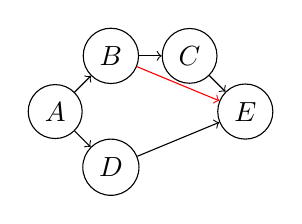
\begin{tikzpicture}[main/.style = {draw, circle}] 
        \node[main] (1) {$A$}; 
        \node[main] (2) [above right of=1] {$B$};
        \node[main] (3) [below right of=1] {$D$}; 
        \node[main] (4) [right of=2] {$C$};
        \node[main] (5) [below right of=4] {$E$}; 
        \draw[->] (1) -- (2);
        \draw[->] (1) -- (3);
        \draw[->] (2) -- (4);
        \draw[->] (4) -- (5);
        \draw[->] (3) -- (5);
        \draw[red, ->] (2) -- (5);
        % \draw[red, ->] (1) -- (4);
    \end{tikzpicture} 
    \caption{Sub-optimality of Original Criteria}
    \label{fig:ex}
    \end{subfigure}
    \begin{subfigure}{0.49\textwidth}
\centering
\begin{tikzpicture}[node distance=2.5cm, every node/.style={font=\small}]
    % Nodes
    \node[circle, draw] (A) {A};
    \node[ellipse, draw, minimum width=3cm, minimum height=1cm, right of=A] (middle) {Set of nodes};
    \node[circle, draw, right of=middle] (C) {C};

    % Dashed path through middle
    \draw[dashed, ->] (A) -- (middle);
    \draw[dashed, ->] (middle) -- (C);

    % Dotted shortcut from A to B
    \draw[dash dot, ->] (A) to[bend right=40] (C);
\end{tikzpicture}
\caption{New maximal-NL PNPS after edge addition}
\label{fig:pr}
\end{subfigure}
\caption{Illustrative example supporting the proof of the DSPG synthesis criteria}
\end{figure}


\begin{theorem}[Soundness and Completeness]
\label{thm:optimized-sound}
Let $A \rightarrow B$ be a candidate branch.

\begin{enumerate}
    \item If the branch satisfies the optimized criteria, the resulting graph remains \ac{DSPG}. \label{thm:firstpart}
    \item If adding the branch does not violate the \ac{DSPG} property, then the branch satisfies the optimized criteria. \label{thm:secondpart}
\end{enumerate}
\end{theorem}

\begin{proof}
This proof is based on the logical structure outlined in Lemma~\ref{lemma}

For \ref{thm:firstpart}: We know that if $A$ is an intermediate node of a PNPS $p$ then $B$ is an intermediate node of $p$ and if $B$ is an intermediate node of a PNPS $p$ then $A$ is an intermediate node of $p$ implies that the DSPG property not broken. What we need to show in this proof is that adding an edge from the source to an intermediate node or from an intermediate node to the sink inside a PNPS $p$ with maximum Nesting Level does not affect the DSPG property of the graph. We are doing the proof for the maximum NL because it is the same as doing the proof for any PNPS since what we want to know is whether we can still reduce a PNPS to a single edge using the DSPG analysis algorithm depicted in Figure~\ref{fig:algsynth2}. During the reduction process, the reduction will be done for this PNPS when the PNPS will be the most nested (the PNPS with maximum Nesting Level).
    \begin{itemize}
        \item add an edge from the source $A$ to an intermediate node $C$:
        Assuming that the current PNPS has max NL, adding this branch does not break the DSPG property because after adding this branch the max NL will be increased by one. Then the new PNPS with maximum NL will be the new one created  $[A,C]$. This new PNPS will be like Figure~\ref{fig:pr} because it is clear that there is only one path from $A$ to $C$ otherwise $A$ and $C$ would have been the source and sink of a PNPS with NL greater than NL of $p$.
    
        \item add an edge from an intermediate node $C$ to the target $B$: Same logic as before. We can just reverse the graph and use the same proof.
    \end{itemize}

    
For \ref{thm:secondpart}: $A$ to $B$ does not break DPSG property. Assuming that the first criterion of criteria defined in \cref{cor:pnps-criteria} is fulfilled, then \cref{prop:dspg} implies that $A$ to $B$ fulfilled Criterion 2 of the optimized Criteria for DSPG Synthesis.
\end{proof}
% \paragraph{Nesting-Level Formulation}

The optimized criteria admit a simple arithmetic restatement in terms of \ac{NNL}.

\begin{theorem}[\ac{NNL} Reformulation of the Optimized Criteria]
\label{thm:nnl-reformulation}
The optimized criteria are equivalent to:

\begin{itemize}
    \item \textbf{Criterion 1}: A path from $A$ to $B$ exists.
    \item \textbf{Criterion 2}:
    \begin{enumerate}
        \item $|\mathrm{NNL}(A) - \mathrm{NNL}(B)| \leq 1$.
        \item Every intermediate node $C$ between $A$ and $B$ satisfies
        \[
        \mathrm{NNL}(C) \geq \min(\mathrm{NNL}(A), \mathrm{NNL}(B)).
        \] 
    \end{enumerate}
\end{itemize}
\end{theorem}

The only difference from the original criteria is that equality of \acp{NNL} is relaxed to a difference of at most one. This relaxation precisely captures admissible additions from a \ac{PNPS} source to its intermediate nodes or from intermediate nodes to its target.


In summary, the optimized criteria provide three improvements:

\begin{enumerate}
    \item They strictly generalize the original criteria.
    \item They preserve \ac{DSPG} correctness.
    \item They maximize information retention.
\end{enumerate}

These criteria form the logical foundation for the optimized synthesis algorithm presented in the next section.


\section{Optimized \acs{DSPG} Synthesis Algorithm}
\label{sec:optimized_algorithm}

In previous \cref{sec:optimized_criteria}, we established necessary and sufficient conditions under which a branch can be added to a \ac{DSPG} without violating structural constraints. We now present a constructive algorithm that implements these criteria and synthesizes a \ac{DSPG} from an arbitrary directed acyclic graph. The algorithm incrementally builds a \ac{DSPG} by selecting admissible branches according to the optimized criteria while maintaining structural information about  \ac{PNPS} membership.

% \subsection{Algorithm Overview}

Let $G = (V,E)$ be a directed acyclic graph that may not satisfy the DSPG property. The synthesis procedure constructs a subgraph $G' \subseteq G$ that is DSPG-compliant. The key idea is based on previous work~\cite{4622580}:
\begin{enumerate}
    \item Enumerate all source-to-sink paths in $G$.
    \item Initialize $G'$ with one valid path.
    \item Iteratively attempt to add remaining branches.
    \item Accept a branch if and only if it satisfies the optimized criteria.
\end{enumerate}

To efficiently evaluate structural conditions, we maintain a mapping
\[
nodeToPNPS : V \rightarrow \{\text{highest nested  \ac{PNPS} containing the node}\}.
\]

This mapping allows constant-time verification of \ac{PNPS} containment constraints.

% \subsection{Algorithm Description}

Algorithm~\ref{alg:dspg-synth} presents the synthesis procedure.
\begin{algorithm}[H]
\caption{Optimized DSPG Synthesis}
\label{alg:dspg-synth}
\begin{algorithmic}[1]
\Require Directed acyclic graph $G = (V,E)$
\Ensure DSPG subgraph $G' \subseteq G$
\State $paths \gets$ GetAllPaths($G$)
\State Sort $paths$ by uncertainty or length
\State $G' \gets$ $paths.pop()$ \Comment{Initialize with first path}
\State $nodeToPNPS \gets \emptyset$
\While{$paths \neq \emptyset$}
    \State $path \gets paths.pop()$
    \State $branch \gets$ first branch of $path$ not in $G'$
    \State $(A,B) \gets (source(branch), target(branch))$
    \State $check \gets$ DSPGChecker($nodeToPNPS$, $A$, $B$)
    \If{$check.bool = \text{True}$}
        \State $G'.addEdges(branch)$

        \State UpdatePNPS($nodeToPNPS$, $check.intermediateNodes$,$branch.intermediateNodes$, $(A,B)$)

    \EndIf
\EndWhile
\end{algorithmic}
\end{algorithm}

\begin{algorithm}
\caption{UpdatePNPS}
\label{alg:update-pnps}
\begin{algorithmic}[1]
\Require $nodesToPNPS$ : current map from node $\rightarrow$ PNPS
\Require branch $BranchListOfIntermediateNodes$
\Require checker $CheckerListOfIntermediateNodes$
\Require $(nodeSource, nodeTarget)$ : candidate PNPS

\Ensure $nodesToPNPS$ maps each node to the **highest nested PNPS** it is part of

\For{$v \in$ $CheckerListOfIntermediateNodes$}
\State $nodesToPNPS[v] \gets smallerPNPS((nodeSource, nodeTarget),\ nodesToPNPS[v])$
\EndFor

\For{v $\in$ $BranchListOfIntermediateNodes$}
\State $nodesToPNPS[v] \gets moreNestedPNPS((nodeSource, nodeTarget),\ nodesToPNPS[v])$
\EndFor

\State \Return $nodesToPNPS$

\end{algorithmic}
\end{algorithm}


The function \texttt{DSPGChecker} verifies the optimized criteria:
\begin{enumerate}
    \item Existence of a path from $A$ to $B$.
    \item Structural containment consistency according to Definition~\ref{def:optimized-criteria}.
\end{enumerate}
\todo[inline]{Add text regarding DSPGChecker algorithm}
\begin{algorithm}
\caption{DSPG Local Checker}
\begin{algorithmic}[1]
\Require Dictionary $\textit{nodesToPNPS}$, source node $src$, target node $target$
\If{there is a path from $src$ to $target$}
    \State $pathNodes \gets$ list of all intermediate nodes in this path
\Else
    \State \Return $\{bool: False\}$
\EndIf

\If{$nodesToPNPS[src] \neq None$}
    \If{$target \notin nodesToPNPS[src]$}
        \State \Return $\{bool: False\}$
    \EndIf
\EndIf

\If{$nodesToPNPS[target] \neq None$}
    \If{$src \notin nodesToPNPS[target]$}
        \State \Return $\{bool: False\}$
    \EndIf
\EndIf

\State \Return $\{bool: True,\; intermediateNodes: pathNodes\}$
\end{algorithmic}
\end{algorithm}

Following we show different properties of the \cref{alg:dspg-synth}.

The correctness of the algorithm relies on the invariant that $nodesToPNPS[v]$ always stores the most deeply nested  \ac{PNPS} in which node $v$ appears as an intermediate node.
\begin{theorem}
Let $a$ and $b$ be two nodes, and assume that we have a mapping 
$nodesToPNPS$ which maps a node to the highest nested PNPS it is part of.
Then we have

\begin{align}
    nodesToPNPS[a] = None \;\text{ or }\; b \in nodesToPNPS[a]
\iff \notag \\
\text{if node } a \text{ is an intermediate node of a PNPS } p
\text{ then } b \text{ is inside } p . \notag 
\end{align}


\end{theorem}
\begin{proof}

($\Rightarrow$)
If $nodesToPNPS[a] = None$, then $a$ is not part of any PNPS.
Therefore the second statement is trivially true.

If $b \in nodesToPNPS[a]$, then $b$ belongs to the most nested PNPS
containing $a$. Since every PNPS containing $a$ also contains
$nodesToPNPS[a]$, it follows that $b$ is part of any PNPS that
contains $a$.

($\Leftarrow$)
If node $a$ is an intermediate node of a PNPS $P$ and $b$ is inside $P$,
then $b$ belongs to every PNPS of which $a$ is an intermediate node.
Since $nodesToPNPS[a]$ represents the most nested PNPS containing $a$,
it follows that $b \in nodesToPNPS[a]$.

\end{proof}

\begin{theorem}
The update of $nodesToPNPS$ in \cref{alg:update-pnps} ensures that $nodesToPNPS$ maps each node to the highest nested PNPS it is part of.
\end{theorem}
\begin{proof}

We want to prove that if before the update of $nodesToPNPS$ the mapping
associates each node with the highest nested PNPS it belongs to,
then after the update this property still holds.

When adding a new branch from $A \to B$, two situations may occur.

\textbf{Case 1:} The subnetwork from $A$ to $B$ was already a PNPS.
In this case, the update only assigns values to the newly added nodes,
while the existing nodes already have the correct mapping.

\textbf{Case 2:} The subnetwork from $A$ to $B$ forms a new PNPS.
Two subcases arise.

\begin{itemize}

\item \textbf{No PNPS between $A$ and $B$.}  
A new PNPS is created. The intermediate nodes of this PNPS are exactly
the nodes on the branch being added and the intermediate nodes on the
path from $A$ to $B$ before adding the branch. These nodes are therefore
updated to map to this newly created PNPS.

\item \textbf{Existing PNPS between $A$ and $B$.}  
Some intermediate nodes on the path from $A$ to $B$ may already belong
to a more nested PNPS. For these nodes, $nodesToPNPS$ is not updated
because they already map to a more nested PNPS. The nodes that are not
part of a more nested PNPS are updated accordingly. This is valid
because every path from $A$ to $B$ before adding the new branch
contains these nodes, meaning they are not intermediate nodes of any
PNPS between $A$ and $B$.

\end{itemize}

Therefore, after the update, each node still maps to the highest nested
PNPS it belongs to.

\end{proof}

\begin{theorem}[Algorithm Soundness]
\label{thm:alg-sound}
At every iteration, $G'$ remains DSPG.
\end{theorem}

\begin{proof}
The algorithm adds a branch only if it satisfies the optimized synthesis criteria of \cref{thm:optimized-sound}. By soundness of those criteria, the addition preserves the DSPG property. Since the initial path is trivially DSPG and each step preserves the invariant, the resulting graph remains DSPG.
\end{proof}

\begin{theorem}[Algorithm Completeness]
\label{thm:alg-complete}
If a branch can be added without violating the DSPG property, the algorithm will accept it.
\end{theorem}

\begin{proof}
By completeness of the optimized criteria in \cref{thm:optimized-sound}, any branch that preserves DSPG must satisfy the structural containment conditions. The \texttt{DSPGChecker} verifies exactly these conditions. Therefore admissible branches are not rejected.
\end{proof}

% \subsection{Termination}

\begin{theorem}[Termination]
\label{thm:termination}
The algorithm terminates after a finite number of iterations.
\end{theorem}

\begin{proof}
The number of paths in a finite directed acyclic graph is finite. At each iteration, one path is removed from the list and processed. No path is reinserted. Therefore the algorithm terminates.
\end{proof}

% \subsection{Complexity Considerations}

Let $P$ denote the number of source-to-sink paths in $G$.

\begin{itemize}
    \item Path enumeration is exponential in the worst case.
    \item Each branch verification is constant time assuming $nodeToPNPS$ is maintained efficiently.
    \item  \ac{PNPS} updates are linear in the size of the branch.
\end{itemize}

Although path enumeration may be expensive in theory, in trust networks the graph structure is typically sparse and limited in depth. Moreover, synthesis is performed once prior to trust inference, making preprocessing cost acceptable.

% \subsection{Structural Implications}

This completes the structural synthesis component of the framework. In the next section, we turn to optimized DSPG analysis and \acp{NL} computation during reduction.

\section{Optimized \acs{DSPG} Analysis and \acs{PNPS}-Based Reduction}
\label{sec:optimized_analysis}

Once a \ac{DSPG} graph has been synthesized, trust inference proceeds through structural reduction. Classical \ac{DSPG} analysis reduces the graph recursively by collapsing \ac{PPS} into single edges until only one edge remains between the global source and sink.

In this section, we demonstrate that replacing \ac{PPS} with  \ac{PNPS} leads to a more stable and structurally isolated reduction process. We formalize the reduction procedure and analyze nesting-level evolution.

% \subsection{PNPS-Based Reduction Principle}

In the classical formulation, a \ac{DSPG} is recursively reduced using two operations:
\begin{enumerate}
    \item Series reduction, which collapses two consecutive edges incident to a node of degree two.
    \item Parallel reduction, which collapses parallel edges into a single edge.
\end{enumerate}

\todo[inline]{the following is not clear at all} In the \ac{PPS}-based framework, identifying valid parallel structures may require global structural reasoning. Furthermore, nesting-level updates are implicitly derived and can be difficult to track precisely.





Using \ac{PNPS}, reduction becomes structurally localized.
\begin{definition}[ \ac{PNPS} Reduction]
Let $P$ be a  \ac{PNPS} with source $A$ and target $B$. A  \ac{PNPS} reduction replaces the entire subnetwork $P$ with a single edge $(A,B)$ whose subjective opinion equals the fusion of the discounted opinions along the paths in \(P\).
\end{definition}

The key advantage of \ac{PNPS} is that structural isolation is guaranteed by Definition~\ref{def:pnps} (\cref{fig:pnps}). Since the parallel paths are node-disjoint, collapsing the subnetwork does not create unintended structural interactions.

Reduction proceeds by iteratively selecting a \ac{PNPS} with maximum \ac{NL}.


The optimized analysis algorithm relies on the fact that reducing a  \ac{PNPS} preserves structural consistency and updates \acp{NL} in a controlled manner.

\begin{theorem}[\ac{PNPS}  Reduction Preservation and Nesting Update]
\label{thm:pnps-reduction}
Let $G$ be a \ac{DSPG}, and let $\text{pnps}_1$ be a \ac{PNPS} in $G$ with the maximum Nesting Level. Then:
\begin{enumerate}
    \item \textbf{(Isolated Transformation)} Transforming $\text{pnps}_1$ into a single edge does not affect the Nesting Level of any other PNPS in the graph.
    \item \textbf{(Nesting Level Update)} The edge that replaces $\text{pnps}_1$ has a Nesting Level equal to $\text{NL}(\text{pnps}_1) - 1$.
\end{enumerate}
\end{theorem}
The theorem formalizes two essential properties.

First, reduction is isolated. The transformation of a maximally nested  \ac{PNPS} does not alter the structural hierarchy of remaining  \acp{PNPS}.

Second, \acp{NL} decrease in a strictly controlled manner. This guarantees termination of the reduction process and preserves ordering among nested structures.


The proof of \cref{thm:pnps-reduction} relies on structural relationships between nested  \acp{PNPS}.

Before proving Theorem~\ref{thm:pnps-reduction}, we need to introduce several elementary results that characterize the structural relationships between nested PNPSs. These results are necessary to justify both the isolation property and the nesting level update described above.
\begin{theorem}
\label{thrm:anlsys1}
\label{thrm:anlsys2}
Consider a DSPG and two PNPSs, $pnps_1$ and $pnps_2$, such that $NL(pnps_1) > NL(pnps_2)$. Then:
\begin{enumerate}
    \item \label{thm:p1} If a node $s$ is the common source of both $pnps_1$ and $pnps_2$, then $s$ must have at least one outgoing edge that is in $pnps_2$ but not in $pnps_1$.
    \item \label{thm:p2} If a node $t$ is the common target of both $pnps_1$ and $pnps_2$, then $t$ must have at least one incoming edge that is in $pnps_2$ but not in $pnps_1$.
\end{enumerate}
\end{theorem}

\begin{proof}
\label{prf:anlsys1}
For part~\ref{thm:p1} of the theorem.
If $NL(pnps_1) > NL(pnps_2)$, then $pnps_1$ and $pnps_2$ don't have the same target (since they already have the same source). Thus:
\begin{itemize}
    \item  either $pnps_1$ is inside $pnps_2$: If $s$ does not have at least one outgoing edge to a node which is inside $pnps_2$ and outside $pnps_1$ it means that all paths from $s$ to target of $pnps_2$ will be through $pnps_1$ since from an intermediate node of $pnps_1$ we cannot go outside $pnps_1$ without reaching the target of $pnps_1$. The consequence is that we will not be able to find two non-intersecting paths therefore the graph is not DSPG;
    
    \item or $pnps_1$ is not inside $pnps_2$ and $Nodes(pnps_1) \cap Nodes(pnps_1) \neq \{s\}$: In this case the graph cannot be a DSPG because it means that $pnps_1$ has an intermediate node $n_1$ inside $pnps_2$ (which are not $s$) and a node $n_2$  outside $pnps_2$. $n_2$ is an intermediate node of $pnps_2$ (otherwise it’s the target node of $pnps_2$, and in this case it impossible to have $NL(pnps_1)>NL(pnps_2 )$). Therefore, from $n_1$ (intermediate node of $pnps_2$) we can reach $n_2$ (outside $pnps_2$)  without visiting the target of $pnps_2$
    
    \item or $pnps_1$ is not inside $pnps_2$ and $Nodes(pnps_1) \cap Nodes(pnps_1) = \{s\}$: In this case $s$ has at least one outgoing edge to a node which is inside $pnps_2$ and outside $pnps_1$ 
    
\end{itemize}

The part~\ref{thm:p2} of the theorem is the dual case of item. Reverse the graph and apply the same reasoning.
\end{proof}

\begin{figure}
    \centering
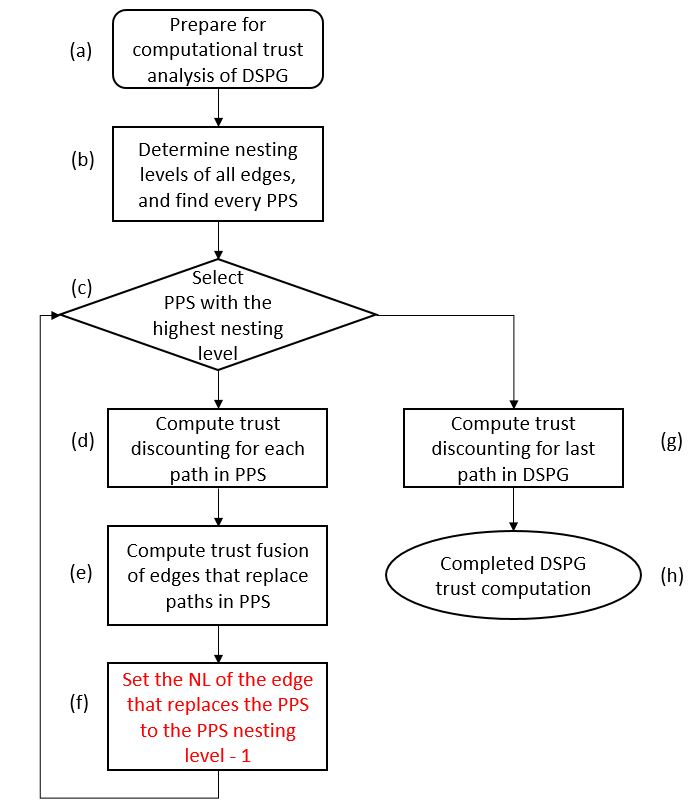
\includegraphics[width=0.5\textwidth]{img/dspg/newsynth.pdf}
    \caption{Our optimized DSPG analysis algorithm}
    \label{fig:algsynth2}
\end{figure}
\begin{corollary}
\label{corol:synth}
Considering a DSPG, if a PNPS $pnps_1$ is nested in another PNPS $pnps_2$ and $pnps_1 \neq pnps_2$, then $pnps_2$ has at least one edge not in $pnps_1$.
\end{corollary}
\begin{proof}
    If a PNPS $pnps_1$ is nested in another PNPS $pnps_2$, we can distinguish between two cases:
\begin{enumerate}
    \item $pnps_1$ and $pnps_2$ do not share the same source and also do not share the same target nodes: if they don't have the same source then the path from the source of $pnps_2$ to the source of $pnps_1$ contains edges outside $pnps_1$. Same reasoning  if they don't have the same target.
    \item $pnps_1$ shares the source or the target (or both) with $pnps_2$: application of Theorems \cref{thrm:anlsys1}.
\end{enumerate}
\end{proof}


We now return to the proof of \cref{thm:pnps-reduction} stated above. 
\begin{proof}
    When reducing a PNPS with the maximum Nesting Level (denoted as $pnps_1$), two structural cases arise:
\begin{enumerate}
    \item $pnps_1$ is a non nested PNPS, or
    \item $pnps_1$  is nested within another PNPS (denoted as $pnps_2$).
\end{enumerate}
In case (1), $pnps_1$ has a Nesting Level equal to 1. After its reduction, all other PNPSs remains the same and the resulting edge has a Nesting Level of 0. In the case (2), since at least one edge --- denoted as $e$ --- in $pnps_2$ is not part of $pnps_1$ (Corrolary~\ref{corol:synth}), $NL(e)$ will remain unchanged and we select it such that its Nesting Level equals that of $pnps_2$ (this follows from  \cref{thrm:anlsys1} with $pnps_1$ Nesting Level equals $pnps_2$ Nesting Level plus 1. Such a PNPS($pnps_2$) exists, as the Nesting Level increments one by one). As a result, the Nesting Level of $pnps_1$ is preserved, since the new edge has Nesting Level reduced by one which is still greater than or equal to that of $pnps_2$.
\end{proof}

\begin{theorem}[Reduction Ordering]
\label{thm:reduction-ordering}
Let $G$ be a DSPG. Reducing a  \ac{PNPS} with maximum \ac{NL} preserves the nesting structure of all remaining  \acp{PNPS}.
\end{theorem}

\begin{proof}
This follows directly from \cref{thm:pnps-reduction}. A maximally nested  \ac{PNPS} is structurally contained within no other \ac{PNPS} of higher \ac{NL}. Therefore its reduction does not modify the structural boundaries of less nested  \acp{PNPS}.
\end{proof}

This ordering guarantees that reduction progresses from the most deeply nested structures outward, ensuring structural consistency.








\subsection{Correctness and Implications for Trust Inference}

Replacing PPS with\ac{PNPS} produces three fundamental improvements:

\begin{enumerate}
    \item \textbf{Stronger isolation guarantees.}  \ac{PNPS} ensures that intermediate nodes cannot connect to external structures without violating DSPG.
    
    \item \textbf{Simplified detection of non-DSPG patterns.} Structural violations become local and verifiable through \cref{prop:dspg}.
    
    \item \textbf{Stable nesting updates.} \cref{thm:pnps-reduction} guarantees predictable nesting-level evolution during reduction.
\end{enumerate}

These properties form the structural backbone of the optimized synthesis and analysis framework presented in the next sections.


\begin{theorem}[Correctness of \ac{PNPS}-Based Reduction]
\label{thm:analysis-correct}
Let $G$ be a DSPG. Iterative \ac{PNPS}-based reduction yields a single edge between the global source and sink whose opinion equals the trust inference result defined by Subjective Logic operators.
\end{theorem}

\begin{proof}
Since every DSPG can be reduced by successive series and parallel reductions, and since  \ac{PNPS} is a stricter form of PPS that preserves structural equivalence, every PPS reduction step is captured by a \ac{PNPS} reduction.

At each reduction step, subjective opinions are combined using valid fusion and discount operators. Because  \ac{PNPS} structures are node-disjoint, operator application is well-defined and free of ambiguity.

Since \acp{NL} decrease strictly and the graph is finite, the process terminates with a single edge representing the global trust evaluation.
\end{proof}


The \ac{PNPS}-based approach improves classical analysis in three aspects:

\begin{enumerate}
    \item \textbf{Structural isolation.} Node-disjointness guarantees reduction does not affect unrelated structures.
    \item \textbf{Deterministic nesting updates.} \acp{NL} decrease in a controlled and predictable manner.
    \item \textbf{Simplified detection.} Structural violations can be identified locally using \cref{prop:dspg}.
\end{enumerate}

In contrast, PPS-based reduction may require global reasoning to ensure that intermediate nodes do not create unintended structural exits.



The \ac{PNPS}-based reduction framework guarantees that:

\begin{itemize}
    \item Every reduction step corresponds to a valid trust operator application.
    \item No structural ambiguity arises during fusion.
    \item Information retention achieved during synthesis is preserved during analysis.
\end{itemize}

This completes the structural component of the optimized framework. We now turn to the operator-level limitation identified previously.








\section{Trust Discounting for Referral Paths}
\label{sec:referral_path_operator}

In DSPG Analysis, trust propagation along referral paths plays a central role in deriving consistent opinions between distant nodes. While classical trust discounting operators allow the combination of a referral edge with a functional edge, they do not guarantee consistency when multiple referral edges appear consecutively in a path. In particular, the projected probability of the resulting opinion is not always equal to the product of the projected probabilities along the path. This limitation becomes critical when reducing  \ac{PNPS} structures, where multi-edge referral chains frequently arise.

To address this issue, we introduce a new \emph{Referral-Edge Path Trust Discounting Operator}, denoted by $\otimes_{RE}$. 
This operator enables consistent trust propagation over two or more consecutive referral edges while preserving probabilistic coherence.

\begin{definition}[Referral-Edges Trust Discountion]
    Let $\omega_B^A = (b_B^A, d_B^A, u_B^A, a_B^A)$ denote the referral trust opinion of agent $A$ about agent $B$, and let $\omega_C^B = (b_C^B, d_C^B, u_C^B, a_C^B)$ denote the referral trust opinion of $B$ about $C$. 

The resulting propagated opinion of $A$ about $C$ through $B$ is defined as:

\begin{align}
\label{equ:tdr_dissertation}
\omega_C^{[A;B]} = \omega_B^A \otimes_{RE} \omega_C^B:
\begin{cases}
b_C^{[A;B]} &= b_B^A \, b_C^B \\
d_C^{[A;B]} &= b_B^A \, d_C^B \\
u_C^{[A;B]} &= 1 - \left( b_C^{[A;B]} + d_C^{[A;B]} \right) \\
a_C^{[A;B]} &= 
\displaystyle
\frac{(b_B^A + u_B^A a_B^A)(b_C^B + u_C^B a_C^B) - b_B^A b_C^B}
{1 - b_B^A (b_C^B + d_C^B)}
\end{cases}
\end{align}

The belief and disbelief are discounted multiplicatively, while the base rate is adjusted to ensure preservation of projected probability.
\end{definition}

A fundamental property of $\otimes_{RE}$ is that it preserves projected probability multiplicativity along referral paths.

\begin{theorem}[Projected Probability Conservation]
\label{thm:projected_probability_preservation}
Let $P_B^A$ and $P_C^B$ denote the projected probabilities of $\omega_B^A$ and $\omega_C^B$ respectively. Then the projected probability of the discounted opinion satisfies:
\begin{equation}
P_C^{[A;B]} = P_B^A \, P_C^B.
\end{equation}
\end{theorem}

\begin{proof}
By definition of projected probability,
\[
P_C^{[A;B]} = b_C^{[A;B]} + u_C^{[A;B]} a_C^{[A;B]}.
\]
Substituting the expressions from \cref{equ:tdr_dissertation} and simplifying yields:
\[
P_C^{[A;B]} = (b_B^A + u_B^A a_B^A)(b_C^B + u_C^B a_C^B) = P_B^A P_C^B.
\]
\end{proof}

This property guarantees probabilistic consistency across arbitrarily long referral chains in optimized DSPGs.

In DSPG reduction, referral paths may contain more than two edges. Therefore, the operator must be associative to ensure path-independent evaluation.

\begin{theorem}[Associativity over Multi-Edge Referral Paths]
\label{thm:associativity_RE}
The operator $\otimes_{RE}$ is associative. For any referral chain $A \rightarrow B \rightarrow C \rightarrow D$, the following holds:
\begin{equation}
(\omega_B^A \otimes_{RE} \omega_C^B) \otimes_{RE} \omega_D^C
=
\omega_B^A \otimes_{RE} (\omega_C^B \otimes_{RE} \omega_D^C).
\end{equation}
\end{theorem}

\begin{proof}
The belief component on both sides equals $b_B^A b_C^B b_D^C$, and the disbelief component equals $b_B^A b_C^B d_D^C$. Since projected probability multiplicativity holds recursively, both expressions yield identical projected probabilities. Given equality of belief, disbelief, and projected probability, uncertainty and base rate coincide. Therefore, the two expressions are equal.
\end{proof}

Associativity ensures that trust propagation over referral chains in optimized DSPGs is independent of grouping, which is essential for \ac{PNPS}-based reductions.

% \subsection{Non-Idempotency}
\begin{theorem}[Referral-Edges Trust Discounting Idempotence]
    The operator $\otimes_{RE}$ is non-idempotent. 
    For an opinion $\omega = (b,d,u,a)$,
    
    \[
    \omega \otimes_{RE} \omega = \omega
    \quad \Longleftrightarrow \quad
    b = 1 \text{ or } (u = 1 \text{ and } a = 1).
    \]
    
\end{theorem}

This property reflects the fact that repeated referral propagation accumulates uncertainty unless the opinion corresponds to absolute belief or total vacuity.

% \subsection{Interpretation in Optimized DSPGs}

Within an optimized \ac{DSPG}, referral edges represent meta-trust relationships between nodes. The operator $\otimes_{RE}$ enables consistent reduction of multi-edge referral paths into a single equivalent edge while preserving projected probability semantics. This guarantees that \ac{PNPS}-based reductions performed in \cref{sec:optimized_analysis} do not alter the probabilistic interpretation of trust values.

As a consequence, optimized DSPG synthesis and trust propagation become algebraically coherent, structurally consistent, and probabilistically well-founded.



\section{Evaluation}
\label{sec:eval_tnasl}
\subsection{Evaluation of Optimized \acs{DSPG} Synthesis}
\label{subsec:eval_synthesis}

In Section~\ref{sec:optimized_criteria} we formally proved the correctness and optimal retention properties of the proposed \ac{DSPG} synthesis criteria. In particular, we demonstrated that the \ac{PNPS}-based reduction preserves structural validity while avoiding unnecessary edge elimination. Therefore, the purpose of this evaluation is not to re-establish correctness, but to assess the practical impact of the optimized synthesis on the final derived trust opinions.

Specifically, we investigate how retaining or discarding structurally valid edges influences the uncertainty of the final trust estimate. This analysis highlights the practical benefits of our retention criteria compared to the original synthesis rules.

\paragraph{Experimental Setup}

We consider the trust graph illustrated in Figure~\ref{fig:ex}. 
Using our optimized synthesis criteria, the final derived opinion $\omega_A^E$ is expressed as:

\begin{equation}
\omega_A^E =
\left[
\omega_B^A \otimes 
\left(
    \left(\omega_C^B \otimes \omega_E^C \right) 
    \oplus 
    \omega_E^B
\right)
\right]
\oplus
\left[
\omega_D^A \otimes \omega_E^D
\right]
\end{equation}

Under the original synthesis criteria, the additional edge $\omega_E^B$ is discarded, yielding:

\begin{equation}
\omega_A^E =
\left[
\omega_B^A \otimes 
\left(
    \omega_C^B \otimes \omega_E^C
\right)
\right]
\oplus
\left[
\omega_D^A \otimes \omega_E^D
\right]
\end{equation}

To quantify the impact of retaining the edge $\omega_E^B$, we vary its uncertainty while keeping all other opinions fixed to 
\[
\left(\frac{1}{3}, \frac{1}{3}, \frac{1}{3}\right).
\]
We set
\[
\omega_E^B = (b, b, u)
\]
and analyze how the final uncertainty of $\omega_A^E$ evolves as $u$ increases from $0$ to $1$.

Figure~\ref{fig:uncertainty_curves} presents the resulting uncertainty curves under two different fusion operators.

\begin{figure}[h!]
    \centering
    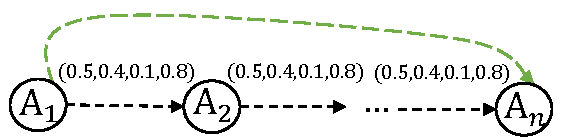
\includegraphics[width=0.4\textwidth]{img/discount/rs2.pdf}
    \caption{Generic referral path with the same numerical opinion for each edge}
    \label{fig:rs2}
\end{figure}

\begin{figure}
    \centering
    \begin{subfigure}{0.45\textwidth}
        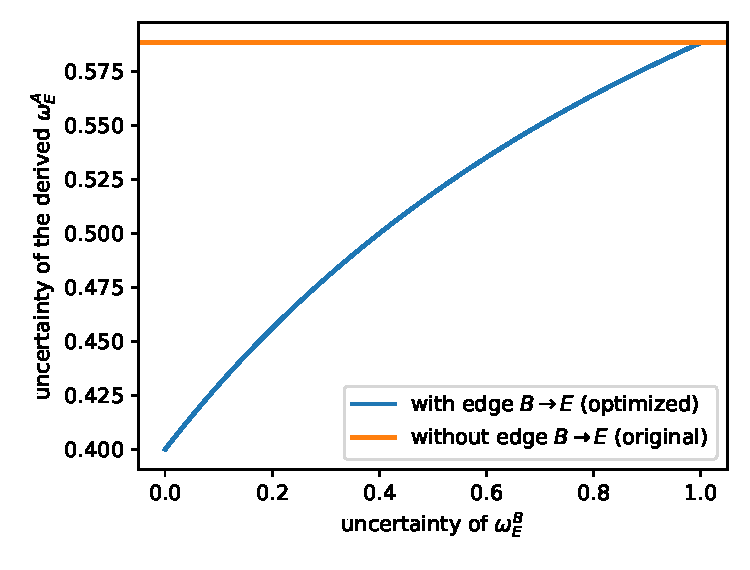
\includegraphics[width=\textwidth]{img/dspg/evalCum.pdf}
        \caption{Impact of edge $B \rightarrow E$ using cumulative fusion}
    \end{subfigure}
    \hfill
    \begin{subfigure}{0.45\textwidth}
        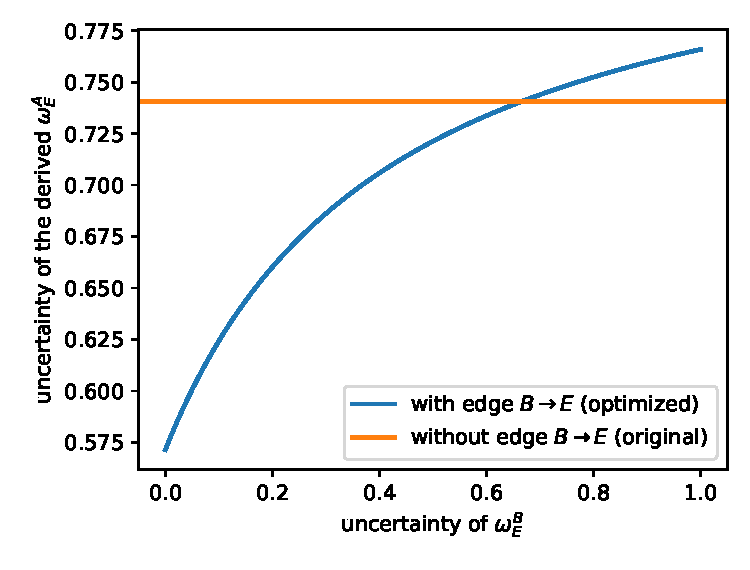
\includegraphics[width=\textwidth]{img/dspg/evalAvg.pdf}
        \caption{Impact of edge $B \rightarrow E$ using averaging fusion}
    \end{subfigure}
    \caption{Impact of retaining edge $B \rightarrow E$ on the uncertainty of the final derived opinion under different fusion operators}
    \label{fig:uncertainty_curves}
\end{figure}

\paragraph{Cumulative Fusion.}

When cumulative fusion is used, including the additional edge $\omega_E^B$ consistently lowers the uncertainty of the final opinion $\omega_A^E$, even when $\omega_E^B$ is highly uncertain. This behavior reflects the cumulative nature of the operator: additional independent evidence, even if partially uncertain, reduces overall uncertainty. Discarding $\omega_E^B$ therefore removes useful supporting evidence and leads to uniformly higher uncertainty.

\paragraph{Averaging Fusion.}
With averaging fusion, the effect depends on the uncertainty level of $\omega_E^B$. When $u(\omega_E^B)$ is small, retaining the edge reduces the final uncertainty. As $u(\omega_E^B)$ approaches $1$, the contribution of $\omega_E^B$ becomes increasingly detrimental, eventually producing higher uncertainty than the case where the edge is removed. This illustrates that averaging fusion is more sensitive to low-quality inputs. However, eliminating structurally valid edges still discards potentially informative trust paths.

These results confirm the practical relevance of the optimized DSPG synthesis criteria. Although minimizing uncertainty alone is not a sufficient objective, preserving structurally valid trust edges ensures that all meaningful trust evidence is retained. The optimized criteria therefore improve inference robustness by preventing premature information loss while maintaining structural correctness.


\subsection{Evaluation of \acs{DSPG} Analysis }
\todo[inline]{Evaluate the Time}
\subsection{Evaluation of Referral-Edge Trust Discounting}
\label{subsec:eval_referral}

\begin{figure}
    \centering
    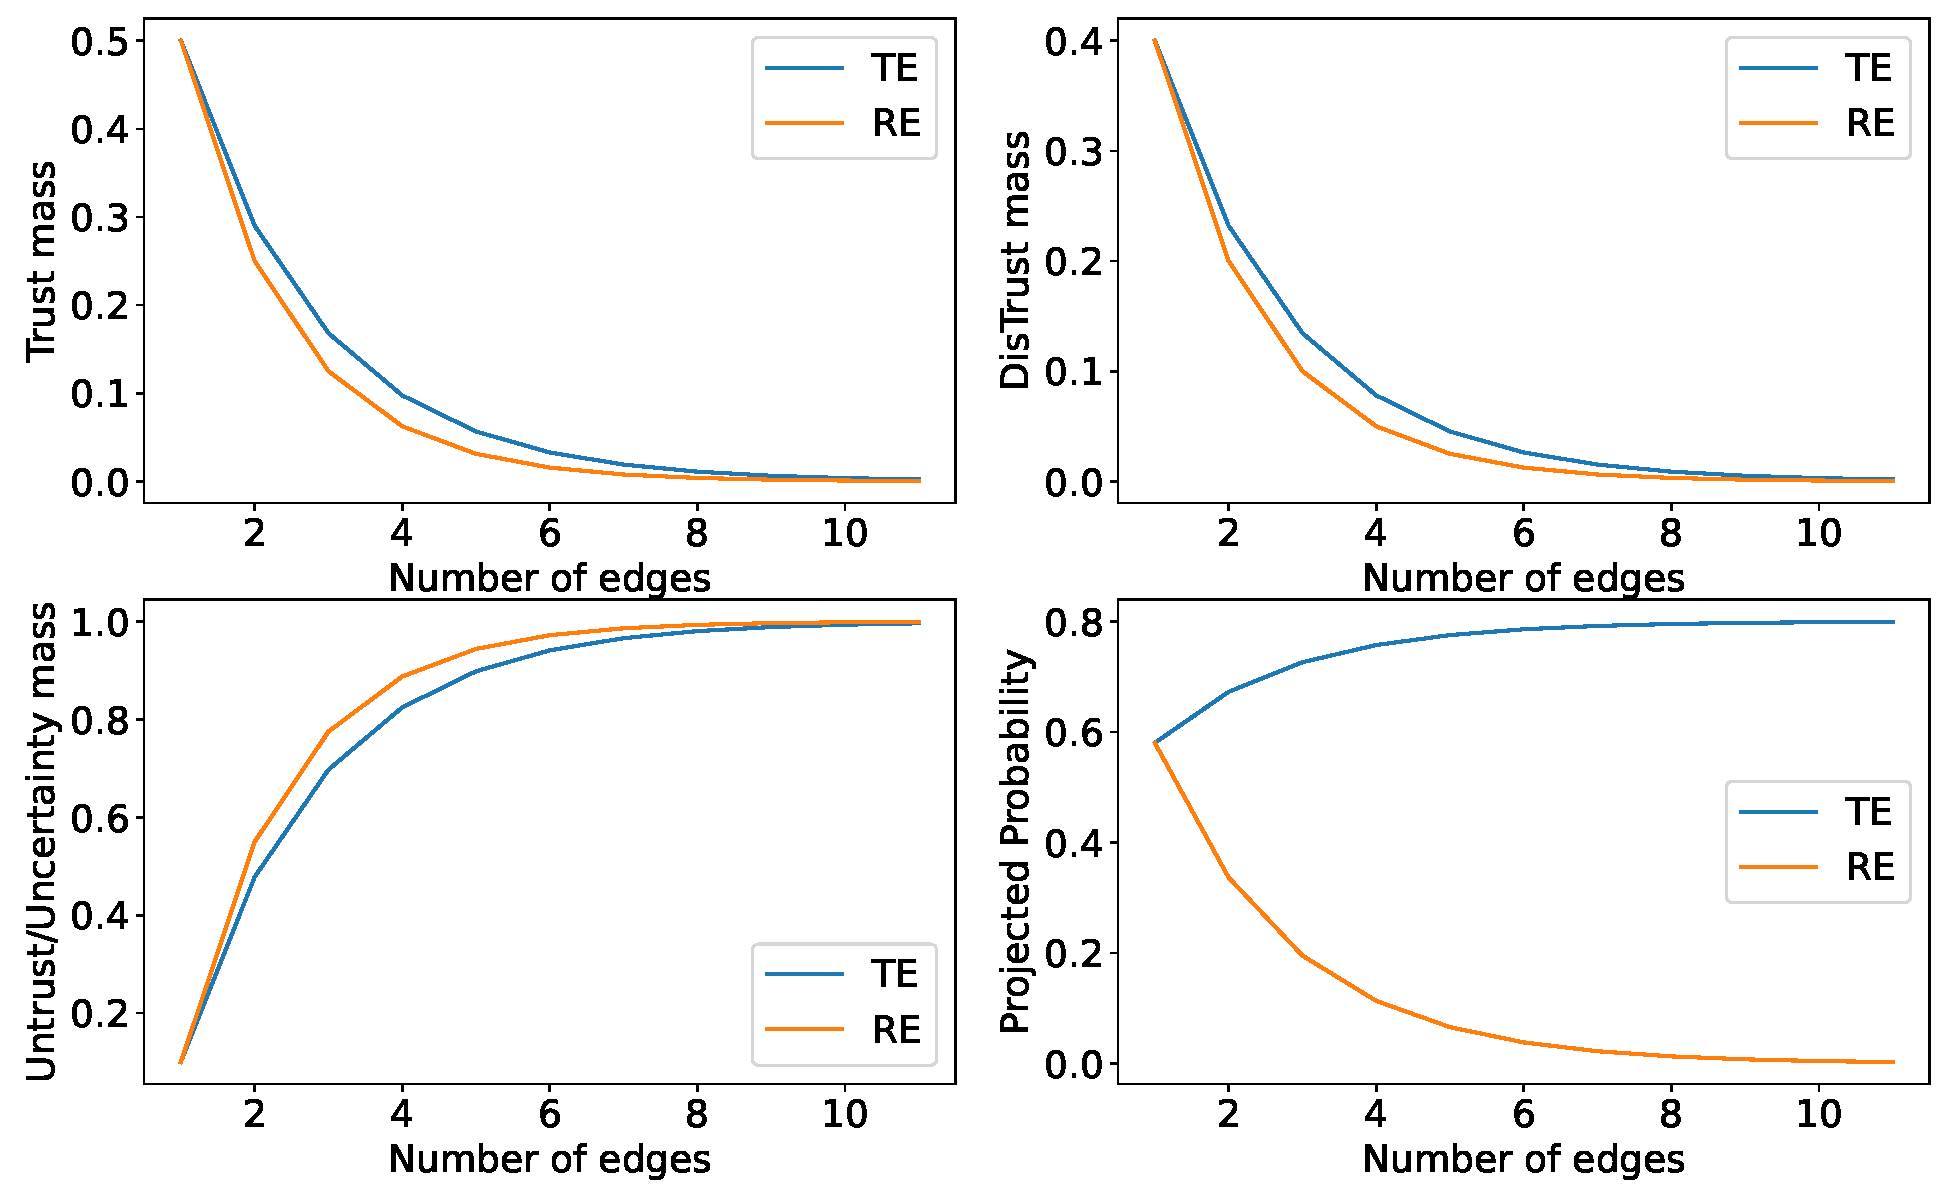
\includegraphics[width=0.8\textwidth]{img/discount/eval.pdf}
    \caption{Comparison of discounting referral edges using Two-Edge Path operator (TE) and the new operator, Referral-Edge Path (RE) on a transitive graph consisting in a varying number of referral edges with all edges having the same trust opinion: (0.5, 0.4, 0.1, 0.8) as depicted in~\cref{fig:rs2}. }
    \label{fig:eval}
    \vspace*{-0.4cm}
\end{figure}


In Section~\ref{sec:meth}, we analytically proved the equivalence between two methods for computing trust over multi-edge referral paths: 

\begin{itemize}
    \item Method 1: Multi-Edge Path discounting.
    \item Method 2: Referral-Edge Path discounting followed by Two-Edge Path discounting.
\end{itemize}

The goal of this section is to numerically validate this equivalence and to illustrate the limitations of the classical Two-Edge Path operator when applied to multiple referral edges.

\subsubsection{Comparison with Multi-Edge and Two-Edge Operators}

We consider the STN depicted in Figure~\ref{fig:rs1}. The following experimental setups are evaluated:

\begin{description}
    \item[Setup 1] Computation of $\omega_X^A$ using the Multi-Edge Path operator (Method 1).
    \item[Setup 2] Computation of $\omega_X^A$ using Referral-Edge Path operator followed by Two-Edge Path operator (Method 2).
    \item[Setup 3] Computation of $\omega_X^A$ using the Two-Edge Path operator applied twice.
\end{description}

\paragraph{Validation of Analytical Equivalence}

Using the opinion values from Figure~\ref{fig:rs1}, we obtain:

\begin{enumerate}
    \item Setup 1:
    \[
    \omega_X^A 
    =
    [\omega^A_B; \omega^B_C] \otimes_{ME} \omega^C_X
    =
    (0.14, 0.07, 0.79)
    \]

    \item Setup 2:
    \[
    \omega_X^A
    =
    (\omega_B^A \otimes_{RE} \omega_C^B) \otimes_{TE} \omega_X^C
    =
    (0.14, 0.07, 0.79)
    \]
\end{enumerate}

The identical numerical results confirm the analytical equivalence established earlier. The proposed operator therefore preserves the semantics of the Multi-Edge Path operator when used in combination with Two-Edge discounting.

\paragraph{Demonstrating the Limitation of Two-Edge Discounting}

We now apply Setup 3, where the Two-Edge Path operator is used to discount two referral edges:

\[
\omega_X^A
=
(\omega_B^A \otimes_{TE} \omega_C^B) \otimes_{TE} \omega_X^C
=
(0.22, 0.11, 0.67)
\]

This result differs significantly from Setups 1 and 2. 

This numerical inconsistency confirms that the Two-Edge Path operator cannot be applied iteratively to referral edges. It lacks associativity and does not preserve projected probability multiplicativity over referral chains. This validates the necessity of the proposed Referral-Edge Path operator.

\subsubsection{Evaluation on Generic Referral Chains}

To further analyze operator behavior, we consider the generic referral path illustrated in Figure~\ref{fig:rs2}. The path contains only referral edges, each assigned the identical opinion:

\[
(0.5, 0.4, 0.1, 0.8)
\]

The number of intermediate nodes varies, allowing us to observe how belief, disbelief, uncertainty, and projected probability evolve as the referral path length increases.

We compare:

\begin{itemize}
    \item Referral-Edge Path operator (RE)
    \item Two-Edge Path operator (TE)
\end{itemize}

The cumulative expressions are:

\begin{align}
\omega^{A_1}_{A_n}
&=
((\omega^{A_1}_{A_2} \otimes_{RE} \dots )
\otimes_{RE}
\omega^{A_{n-2}}_{A_{n-1}})
\otimes_{RE}
\omega^{A_{n-1}}_{A_n}
\label{eq:RE_eval}
\end{align}

\begin{align}
\omega^{A_1}_{A_n}
&=
((\omega^{A_1}_{A_2} \otimes_{TE} \dots )
\otimes_{TE}
\omega^{A_{n-2}}_{A_{n-1}})
\otimes_{TE}
\omega^{A_{n-1}}_{A_n}
\label{eq:TE_eval}
\end{align}

Since the Two-Edge operator is not associative, different grouping strategies yield different results. For consistency, we follow a fixed left-to-right grouping.

\paragraph{Observed Behavior}

Figure~\ref{fig:eval} illustrates the evolution of belief, disbelief, uncertainty, and projected probability as the path length increases.

For both operators:

\begin{itemize}
    \item Belief decreases.
    \item Disbelief decreases.
    \item Uncertainty increases.
\end{itemize}

However, their projected probability behaviors differ fundamentally:

\begin{itemize}
    \item For the Referral-Edge operator, projected probability decreases toward zero as the path length increases.
    \item For the Two-Edge operator, projected probability increases toward the base rate value $0.8$.
\end{itemize}

\paragraph{Analytical Explanation}

From the definitions of the operators:

For Two-Edge discounting:
\[
b^{[A;B]}_C = P_B^A b_C^B
\]

For Referral-Edge discounting:
\[
b^{[A;B]}_C = b_B^A b_C^B
\]

Since the projected probability satisfies:
\[
P_B^A = b_B^A + a_B^A u_B^A \geq b_B^A,
\]

the Two-Edge operator produces larger belief and disbelief components than the Referral-Edge operator. Consequently, the uncertainty mass for Two-Edge discounting is smaller.

This explains why the uncertainty curve for RE lies above TE in Figure~\ref{fig:eval}.

\paragraph{Impact of Base Rate Sensitivity}

Although the Referral-Edge operator produces higher uncertainty, it prevents excessive sensitivity to the base rate.

Under Two-Edge discounting, as uncertainty approaches one and belief and disbelief approach zero, the projected probability converges toward the base rate of the final edge. In this example, this leads to convergence toward $0.8$ for long paths.

This behavior masks the structural weakening of long referral chains.

In contrast, the proposed operator maintains multiplicative projected probability decay. As the number of referral edges increases, the projected probability decreases toward zero. This aligns with the intuition that long referral chains should represent weaker trust.

\paragraph{Interpretation}

The proposed Referral-Edge Path operator therefore satisfies three essential properties:

\begin{enumerate}
    \item Associativity over referral chains.
    \item Preservation of projected probability multiplicativity.
    \item Reduced sensitivity to base rate dominance.
\end{enumerate}

These properties make it structurally and probabilistically coherent for modeling transitive trust in Subjective Trust Networks.


\subsection{End-to-End Evaluation of the Complete \acs{TNA-SL} Framework}
\label{subsec:eval_pipeline}
\section{Summary \& Conclusions}
\label{sec:summary_tnsl}